\chapter{Empirical Evaluation}
\label{ch:hitl}

This chapter reports the thesis's empirical evaluation. It opens with the dataset-curation process behind the IR detector. That detector was co-developed with its training data across five numbered revisions, each driven by the model's own failure modes. The account covers the label-reviewer tool (\S\ref{sec:label_reviewer}), the disciplined loop (\S\ref{sec:hitl_ir}), and the empirical trace on a fixed held-out test split (\S\ref{sec:ir_evolution}). It then evaluates the full system (\S\ref{ch:experiments}).

\section{The Co-Evolution Problem}
\label{sec:coevolution}

A static-corpus detector has a fixed relationship with its training distribution; deployment surfaces shifts that cannot be anticipated at training time. Making the model's own failure modes the primary driver of corpus expansion concentrates annotation effort where marginal value is highest.

Dataset and model state are coupled: a model on corpus $k$ generates errors that define corpus $k+1$, and corpus $k+1$ trains model $k+2$. The coupling is productive when the loop is disciplined, since reviewed errors become clean labels or hard negatives. It turns regressive when it is not: unlabelled positives in an un-reviewed batch enter as confuser-class negatives, as the V5 regression in \S\ref{sec:ir_evolution} illustrates (distinct from the \texttt{mlp\_v5} verifier of \S\ref{sec:distill_verifier}).

\section{Label Reviewer GUI}
\label{sec:label_reviewer}

The label reviewer (\texttt{scripts/label\_reviewer/}) is a PySide6 desktop tool for dataset curation, expanded as the IR-development loop surfaced new failure modes. Its working unit is a candidate frame: an image, the existing GT box(es), and the current model's predicted box(es). For each frame, the reviewer can:

\begin{itemize}
    \item \textbf{Accept GT, reject model} --- GT is correct; the model's disagreement is a FP / FN case logged for analysis.
    \item \textbf{Accept model, override GT} --- the model is correct; the existing GT is missing a box or contains an over-sized / mis-located one. Common in the IR set, where many "missing" GT boxes correspond to small drones the original annotator missed.
    \item \textbf{Adjust the box geometry} --- click-drag editing of corners; addresses the loose-box pattern common in scraped datasets.
    \item \textbf{Re-class} --- for the confuser corpus, where a frame initially flagged as ``drone'' is in fact a bird, airplane, or helicopter to be demoted to a negative.
    \item \textbf{Mark as negative} --- the frame contains no drone; promoted into the hard-negative training set. This is the channel feeding the loop's negative-mining branch.
    \item \textbf{Defer / flag} --- ambiguous frames queued for a second pass rather than forced into a binary decision.
\end{itemize}

Batch operations correct a contiguous segment in one step; filtered views surface only disagreement frames; corrected labels export to YOLO format at session end, with the model acting as a triage layer.

\begin{figure}[htbp]
    \centering
    \fbox{\parbox{0.9\textwidth}{\centering\vspace{2.2cm}
        \textbf{[PLACEHOLDER --- Label reviewer GUI screenshot]} Annotated screenshot of the PySide6 reviewer showing the disagreement-frame view (model box vs.\ GT box in two colours), the box-edit handles, the per-frame action buttons (accept GT / accept model / adjust / re-class / negative / defer), and the side panel that drives the negative-mining branch of the loop.
    \vspace{2.2cm}}}
    \caption{Label reviewer GUI with a Svanstr\"om frame on which V3 fires and the existing GT is missing. The reviewer's two-key resolution path turns the disagreement into either a corrected label (positive ingest) or a hard negative (negative-mining branch).}
    \label{fig:label_reviewer}
\end{figure}

\section{HITL Co-Evolution Loop}
\label{sec:hitl_ir}

Each revision follows the same loop:

\begin{enumerate}
    \item \textbf{Train.} Train the next model version on the current dataset state.
    \item \textbf{Predict.} Run the new model on a candidate pool: held-out validation frames, freshly acquired video, and frames the previous model failed on.
    \item \textbf{Disagree.} Identify model-vs-GT disagreements: (i) model fires on a GT-less frame and is right (missing-annotation FN); (ii) model is silent on a GT frame and is right (spurious-GT FP); (iii) model and GT agree on centre but disagree on box size (loose annotator boxes).
    \item \textbf{Review.} Adjudicate each disagreement via the label reviewer (\S\ref{sec:label_reviewer}). Accept-correct-defer.
    \item \textbf{Identify negative gaps.} Model firings on non-drone scenes (textured clouds, buildings, hot-pixel rows) are promoted to hard negatives in the next training set.
    \item \textbf{Augment.} Apply the corrected labels, append the new positives and negatives, and emit the next dataset version.
\end{enumerate}

\begin{figure}[htbp]
    \centering
    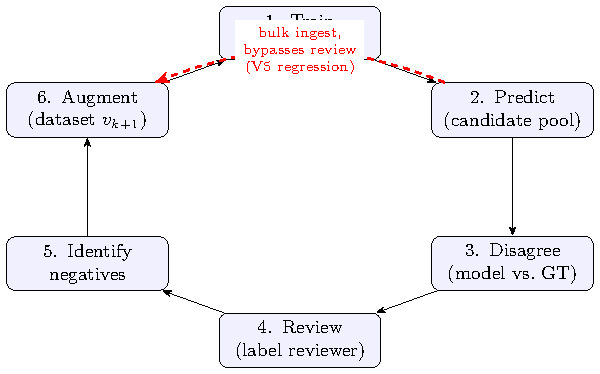
\includegraphics[width=0.62\textwidth]{figures/fig_hitl_loop.pdf}
    \caption{The HITL co-evolution loop. The disciplined path (blue) routes every candidate batch through Disagree$\rightarrow$Review before it is augmented into the next dataset. The V5 regression (\S\ref{sec:ir_evolution}) took the red shortcut: a large positive batch was ingested directly, bypassing review, so unlabelled drones entered training and were scored as false positives.}
    \label{fig:hitl_loop}
\end{figure}

A model FP is either a real error (hard negative needed) or an annotation error (correct the GT); a model FN is either a real miss (hard positive) or a spurious GT box (remove it). Every disagreement is actionable. The empirical record is the precision/recall trace in \S\ref{sec:ir_evolution}.

\section{Case Study: IR Detector Evolution V2 $\to$ Final $\to$ v3b}
\label{sec:ir_evolution}

The IR detector was developed across five numbered revisions (V2 through V6) plus a \texttt{Final} retrain and a \texttt{v3b} corrective fine-tune. Earlier per-version best-epoch mAP50 numbers are not directly comparable because the val split changed with the dataset. Every version was therefore re-evaluated on the same fixed \texttt{IR\_dset\_final} test split at \texttt{imgsz=640} (script: \texttt{eval/eval\_ir\_versions.py}).

\begin{table}[htbp]
    \centering
    \caption{IR detector versions evaluated on the fixed \texttt{IR\_dset\_final} test split @ \texttt{imgsz=640}. Comparable across versions; supersedes the per-version best-epoch mAP narrative. \texttt{v3b} is the production weight; all earlier versions, including \texttt{Final}, are superseded.}
    \label{tab:ir_evolution}
    \begin{tabular}{lcccccc}
        \toprule
        Version & mAP50 & mAP50-95 & $P$ & $R$ & F1 & Status \\
        \midrule
        V2     & 0.458 & 0.219 & 0.661 & 0.406 & 0.503 & superseded \\
        V3     & 0.571 & 0.242 & 0.648 & 0.579 & 0.611 & superseded \\
        V4     & 0.722 & 0.393 & 0.895 & 0.669 & 0.765 & superseded \\
        V5     & 0.694 & 0.446 & 0.768 & 0.709 & 0.737 & superseded (regression) \\
        V6     & 0.956 & 0.571 & 0.921 & 0.941 & 0.931 & superseded \\
        Final  & \textbf{0.977} & \textbf{0.602} & 0.955 & \textbf{0.980} & 0.967 & base for prod \\
        \textbf{v3b (production)} & 0.972 & 0.591 & \textbf{0.957} & 0.977 & \textbf{0.967} & current \\
        \bottomrule
    \end{tabular}
\end{table}

\begin{figure}[htbp]
    \centering
    
\includegraphics[width=0.85\textwidth]{fig4_ir_evolution}
    \caption{IR detector P/R trajectory across the five numbered revisions (V2--V6) plus the \texttt{Final} retrain and production \texttt{v3b}, on the fixed \texttt{IR\_dset\_final} test split. The V5 regression (precision $0.895 \to 0.768$) is recovered by V6 and the production \texttt{v3b}.}
    % [source: ledger=ir-version-progression; eval=ir_final_v3b; run=eval/ir_version_comparison.py; cache=eval/results/ir_version_comparison/ir_comparison_test_640_2026-05-16T20-04-39.csv; config=ir_final_640]
    \label{fig:ir_evolution}
\end{figure}

The trajectory can be read in four passes.

\emph{V2 $\to$ V3: recall-driven gain off a noisier corpus.} V2 was a 300-epoch fine-tune on a broader merged corpus --- the weakest version on every aggregate metric (mAP50 0.458, F1 0.503) though its precision (0.661) exceeds V3's (0.648). V3's narrower curated subset trades a little precision for a large recall gain ($0.406 \to 0.579$), lifting F1 ($0.503 \to 0.611$) and mAP50 ($0.458 \to 0.571$). On this split the curated subset, not the broader merge, is the better training base --- the premise for the FP-mining and split-cleanup cycles that follow.
% [source: ledger=ir-version-progression; eval=ir_final_v3; run=eval/ir_version_comparison.py; cache=eval/results/ir_version_comparison/ir_comparison_test_640_2026-05-16T20-04-39.csv; config=ir_final_640]

\emph{V3 $\to$ V4: precision jump, not a recall jump.} Precision rises from 0.648 to 0.895; recall barely moves (0.579 $\to$ 0.669) --- the signature of an FP-mining cycle.
% [source: ledger=ir-version-progression; eval=ir_final_v4; run=eval/ir_version_comparison.py; cache=eval/results/ir_version_comparison/ir_comparison_test_640_2026-05-16T20-04-39.csv; config=ir_final_640]

\emph{V5 regression.} Precision drops from 0.895 to 0.768 because a large positive batch was injected all at once, bypassing the review loop of \S\ref{sec:hitl_ir}. The un-reviewed batch carried unlabelled drones; V5 fires on them and is scored as FP. V6 and \texttt{Final} are the recovery.
% [source: ledger=ir-version-progression; eval=ir_final_v5; run=eval/ir_version_comparison.py; cache=eval/results/ir_version_comparison/ir_comparison_test_640_2026-05-16T20-04-39.csv; config=ir_final_640]

\begin{figure}[htbp]
    \centering
    \fbox{\parbox{0.9\textwidth}{\centering\vspace{2cm}
        \textbf{[PLACEHOLDER --- V5 regression qualitative]} 3--4 frame panel showing scenes where V4 was correct and V5 fires on newly-ingested but unlabelled drones (scored as FP). Same scenes after corpus cleanup (V6) where the label is corrected and the model fires correctly.
    \vspace{2cm}}}
    \caption{V5 regression case study: same scenes scored as FP under V5 (label missing) and as TP under V6 (label corrected). The model state is unchanged across the V5--V6 transition in these frames; the dataset state is what moved.}
    \label{fig:v5_regression}
\end{figure}

\emph{\texttt{Final} vs v3b are indistinguishable on this split} (both F1$=$0.967). \texttt{v3b} is retained as production because its 2-epoch corrective fine-tune addresses deployment failures (GUI regressions, hot-pixel scenes) not represented in this split.
% [source: ledger=ir-version-progression; eval=ir_final_v3b; run=eval/ir_version_comparison.py; cache=eval/results/ir_version_comparison/ir_comparison_test_640_2026-05-16T20-04-39.csv; config=ir_final_640]

% ======================================================================
% CHAPTER 6 — EXPERIMENTAL RESULTS
% ======================================================================
\section{Experimental Results}
\label{ch:experiments}

\paragraph{Study design.}
The empirical evaluation answers the thesis's three research questions, restated and answered in full in \S\ref{sec:rq_answers}, against the datasets and scoring rules defined earlier. RQ1 (does a downstream cascade suppress the confuser false alarms the detector cannot?) is addressed by the cumulative-suppression and classifier-comparison evaluations (\S\ref{sec:cumulative}); RQ2 (what does that cost in-distribution, and is the cost surface-dependent?) by the Svanstr\"om-versus-real-video exchange (\S\ref{sec:realvideo_cascade}); and RQ3 (does a thermal-trained detector transfer to grayscale RGB?) by the cross-modal real-video diagnostic (\S\ref{sec:grayscale}). The scoring-rule sensitivity that bounds cross-study comparison (\S\ref{sec:scoring_audit}) is treated as a methodological caveat rather than a research question. The unit of analysis is the frame except where a per-clip or per-segment grain is stated, and the in-distribution overlaps that bound each surface are made explicit in the threats analysis (\S\ref{sec:threats}).

Design ablations (classifier variants, patch threshold sweep, catch-rate audit) are in Section~\ref{ch:architecture} \S\S\ref{sec:classifier_compare}--\ref{sec:patch_audit}.

\subsection{Confuser Suppression Across the Cascade}
\label{sec:cumulative}

The cascade is evaluated in three modes: an OOD confuser-zoo mode (no GT; every detection is an FP); a Svanstr\"om paired mode (real GT; IoP@0.5 scored); and a per-classifier comparison. This is the \emph{comparison} configuration that motivated the production picks of \S\ref{sec:production_stack}, not the production stack itself: the figures below use the baseline RGB model, the IR \texttt{v3b} weights, the v2 patch verifier, \texttt{imgsz=1280}, \texttt{rgb\_conf=0.25}, \texttt{ir\_conf=0.40}. The production RGB detector (\texttt{ft4}), trust classifier (\texttt{robust8}), and per-frame verifiers (\texttt{mlp\_v5}/\texttt{mlp\_v5\_ir\_aligned}) are evaluated at the component level in \S\ref{sec:feature_selection} and \S\ref{sec:distill_verifier}; their full-cascade re-run is the registered placeholder of Figure~\ref{fig:mlp_pipeline_placeholder}.
% [source: ledger=cascade-confuser-collapse; eval=clfzoo_fnfn; run=eval/cumulative_halluc.py; cache=eval/results/_cumulative_halluc/confuser_fusion_no_fn_model_v1.1/summary.json; config=confuser_zoo_1280]

\begin{table}[htbp]
    \centering
    \caption{Confuser zoo (no GT, 2,633 OOD imgs). \texttt{fusion\_no\_fn\_v1.1} classifier, v2 patch verifier.}
    \label{tab:cum_confuser}
    \begin{tabular}{lrccc}
        \toprule
        Source & N & S1 fire & S2 fire & S3 fire \\
        \midrule
        AIRPLANE (roboflow) & 99 & 0.273 & 0.030 & 0.030 \\
        OTHER (svan+kaggle+roboflow) & 2,534 & 0.530 & 0.015 & 0.007 \\
        \textbf{OVERALL} & 2,633 & \textbf{0.521} & \textbf{0.016} & \textbf{0.008} \\
        \bottomrule
    \end{tabular}
\end{table}

\begin{figure}[htbp]
    \centering
    
\includegraphics[width=0.75\textwidth]{fig6_1_cumulative_confuser}
    \caption{Cumulative confuser-zoo fire rate across the cascade with the open-world fallback classifier \texttt{fusion\_no\_fn\_v1.1}. The bulk of the suppression is at the classifier stage; the patch verifier roughly halves the residual.}
    \label{fig:cumulative_confuser}
\end{figure}

\begin{table}[htbp]
    \centering
    \caption{Svanstr\"om paired @ \texttt{imgsz=1280}, IoP@0.5, full 28,710 frames. \texttt{fusion\_no\_fn\_v1.1} classifier, v2 patch verifier. Drone class only.}
    \label{tab:cumulative_svanstrom}
    \begin{tabular}{lcccccc}
        \toprule
        Stage & TP & FP & FN & $P$ & $R$ & F1 \\
        \midrule
        S1 RGB alone        & 11260 & 721 & 454 & 0.940 & \textbf{0.961} & 0.950 \\
        S2 + trust classifier & 10682 & 991 & 1032 & 0.915 & 0.912 & 0.914 \\
        S3 + patch v2 (\texttt{thr=0.5}) & 9564 & 756 & 2150 & 0.927 & 0.817 & 0.868 \\
        \bottomrule
    \end{tabular}
\end{table}

\begin{figure}[htbp]
    \centering
    
\includegraphics[width=0.85\textwidth]{fig6_2_svanstrom_by_category}
    \caption{Per-category cascade suppression on Svanstr\"om paired confuser frames. Each confuser category's S1 fire rate drops sharply at the classifier stage; the patch verifier removes the residual on helicopters (near-zero S3) and most of it on birds.}
    \label{fig:svanstrom_by_cat}
\end{figure}

The OOD zoo (Table~\ref{tab:cum_confuser}) measures \emph{confuser-fire reduction}: the classifier carries $\sim$98\% of cumulative suppression and the patch verifier halves the residual. The Svanstr\"om paired evaluation (Table~\ref{tab:cumulative_svanstrom}) measures the \emph{in-distribution cost}: recall suffers ($R: 0.961 \to 0.912 \to 0.817$); precision is roughly stable.
% [source: ledger=cascade-confuser-collapse; eval=clfzoo_fnfn; run=eval/cumulative_halluc.py; cache=eval/results/_cumulative_halluc/confuser_fusion_no_fn_model_v1.1/summary.json; config=confuser_zoo_1280]

With sa32, OOD-zoo fire falls only to 20.5\% (\S\ref{sec:classifier_compare}, Table~\ref{tab:classifiers}) --- an order of magnitude weaker than fnfn but still a 2.5$\times$ reduction --- while Svanstr\"om Stage-3 $F1=0.895$ at $\mathtt{patch\_thr}=0.9$ (\S\ref{sec:patch_threshold}) roughly ties fnfn. The fnfn numbers above are therefore the strongest OOD-suppression case, not the production stack's headline.
% [source: ledger=cascade-confuser-collapse; eval=svan_s3_sa32_thr08; run=(EVIDENCE_LEDGER sweep); config=svan_iop_1280_s9]

The cascade is an exchange: in-distribution F1 for OOD safety. \S\ref{sec:patch_threshold} shows that raising \texttt{patch\_thr} from 0.5 to 0.9 recovers most of the S3 recall loss ($R=0.869$, $F1=0.895$) at a small confuser-FP cost; production ships at \texttt{patch\_thr}$=$0.9. On real video (\S\ref{sec:realvideo_cascade}) the temporal smoother inverts this exchange: the cascade gains drone $F1$ while still cutting confuser FPR threefold. The exchange is therefore a property of the classifier and evaluation surface, not of the cascade architecture.
% [source: ledger=cascade-segment-recovers; eval=svan_s3_sa32_thr08,pipe_vid_baseline_seg; run=(EVIDENCE_LEDGER sweep); config=svan_iop_1280_s9]

\begin{figure}[htbp]
    \centering
    
\includegraphics[width=0.72\textwidth]{fig8_surface_exchange}
    \caption{The cascade's drone-$F1$ exchange is surface-dependent (RQ2). On in-distribution Svanstr\"om-paired data the full cascade \emph{costs} $5.5$~pp drone $F1$ ($0.950\to0.895$, sa32 at \texttt{patch\_thr}=0.9); on operational real video it \emph{gains} $6.6$~pp ($0.760\to0.826$) as temporal smoothing recovers per-frame misses. Same architecture, opposite sign.}
    % [source: ledger=cascade-segment-recovers; eval=rgb_svan_baseline,svan_s3_sa32_thr08,pipe_vid_baseline_seg; run=eval/diagnose_failures.py; config=svan_iop_1280]
    \label{fig:surface_exchange}
\end{figure}
% [source: ledger=trust-classifier-conditional; eval=svan_s3_sa32_thr08; run=(EVIDENCE_LEDGER sweep); config=svan_iop_1280_s9]

\subsection{OOD: Roboflow Audit}
\label{sec:roboflow}

The Roboflow OOD audit evaluates the RGB and IR detectors on nine community datasets at \texttt{imgsz=640}, scored against the datasets' own labels (where present) or counted as pure-FP frames (where none exist). The patch verifier is run as a per-frame filter; the trust classifier is not. The audit therefore measures detector + patch verifier OOD behaviour in isolation.

\subsubsection{Aggregated RGB Drone Performance}

\begin{table}[htbp]
    \centering
    \caption{RGB drone detection across the Roboflow \texttt{rgb\_drone} splits.}
    \label{tab:ood_rgb_drone}
    \begin{tabular}{llccc}
        \toprule
        Model & Stage & $P$ & $R$ & F1 \\
        \midrule
        baseline      & raw           & 0.912 & 0.746 & 0.820 \\
        baseline      & + patch v2    & 0.927 & 0.690 & 0.792 \\
        \texttt{retrained\_v2}  & raw           & 0.924 & 0.726 & 0.813 \\
        \texttt{retrained\_v2}  & + patch v2    & 0.929 & 0.686 & 0.790 \\
        \bottomrule
    \end{tabular}
\end{table}

Two findings. First, the baseline RGB detector wins on OOD drone recall, which indicates that \texttt{retrained\_v2}'s Svanstr\"om collapse is not a generalisable recall defect but resolution-bound (\S\ref{sec:resolution_arch}). Second, the patch verifier costs net F1 on \emph{every} drone setting at \texttt{imgsz=640} ($-2.3$ to $-2.8$~pp): trained on Svanstr\"om-scale crops, its discrimination capacity does not transfer to Roboflow OOD imagery at the same rate as its drone-veto rate.
% [source: ledger=selcom-ood-confuser-damage; eval=rob_rgb_baseline,rob_rgb_retrainedv2; run=eval/run_roboflow_eval.py; config=roboflow_rgb_drone_640]

\subsubsection{Aggregated RGB Confuser FP Suppression}

\begin{table}[htbp]
    \centering
    \caption{Patch verifier RGB confuser FP suppression on Roboflow OOD splits.}
    \label{tab:ood_rgb_confuser}
    \begin{tabular}{lcccc}
        \toprule
        Confuser & baseline supp\% & \texttt{retrained\_v2} supp\% & Total cuts (best) & Notes \\
        \midrule
        airplane   &  3.1\% &  1.9\% &  $\leq$32 & verifier ineffective on OOD airplanes \\
        bird       & 50.5\% & 51.8\% & 52 & verifier transfers well to OOD birds \\
        helicopter & 36.1\% &  8.1\% & 165 & baseline-favored \\
        \bottomrule
    \end{tabular}
\end{table}

The Svanstr\"om-vs-Roboflow airplane suppression gap (52\% vs 3.1\%) is dataset-induced: Svanstr\"om airplanes are predominantly small-and-distant, matching the verifier's training distribution, whereas Roboflow airplanes are typically large-and-close --- a regime underrepresented in training. Bird suppression transfers (50--52\%) because the small-bird regime is consistent across sources. This is the verifier's ``OOD ceiling''.
% [source: ledger=patch-verifier-distribution-bound; eval=rob_rgb_baseline; run=eval/run_roboflow_eval.py; config=roboflow_rgb_drone_640]

\subsubsection{IR Drone and Confuser Performance}

\begin{table}[htbp]
    \centering
    \caption{IR detector on Roboflow OOD drone splits.}
    \label{tab:ood_ir}
    \begin{tabular}{llccc}
        \toprule
        Dataset & Stage & $P$ & $R$ & F1 \\
        \midrule
        \texttt{ir\_drone\_night} & raw & 0.494 & \textbf{0.264} & 0.344 \\
        \texttt{ir\_drone\_night} & + patch v2 & 0.474 & 0.210 & 0.291 \\
        \texttt{ir\_mixed\_cbam}  & raw & 0.821 & 0.519 & 0.636 \\
        \texttt{ir\_mixed\_cbam}  & + patch v2 & 0.874 & 0.491 & 0.628 \\
        \bottomrule
    \end{tabular}
\end{table}

The IR detector has a hidden OOD ceiling. In-distribution recall reaches $R \geq 0.945$; on \texttt{ir\_mixed\_cbam} it drops to $R=0.519$ and on \texttt{ir\_drone\_night} to $R=0.264$. The latter is partly augmentation-induced, but the \texttt{ir\_mixed\_cbam} number is a real generalisation gap (\S\ref{sec:limits}).
% [source: ledger=ir-ood-recall-ceiling; eval=ir_ood_cbam_raw; run=(EVIDENCE_LEDGER sweep); config=roboflow_ir_drone_640]

\subsection{Real-Video Six-Mode Diagnostic}
\label{sec:realvideo}

A real-video diagnostic was conducted on 19 curated YouTube clips: 9 drone-positive (1{,}234 GT drone frames) and 10 confuser-only (1{,}250 frames, no drones), all visually inspected. Six detector modes were compared at \texttt{conf=0.25}, IoP@0.5: the three RGB variants (baseline, \texttt{retrained\_v2}, \texttt{Yolo26n\_selcom\_mixed\_ft2\_1280} at \texttt{imgsz=1280}); the SelCom fine-tune at \texttt{imgsz=640} (\texttt{selcom\_640}) as a resolution ablation; and the IR detector \texttt{v3b} on grayscale-converted or raw RGB.
% [source: ledger=ir-grayscale-fallback; eval=vid_drone_ir_gray; run=eval/eval_video_tests.py; config=video_drone_iop]

\begin{table}[htbp]
    \centering
    \caption{Real-video six-stack diagnostic. Drone columns: aggregate $P$, $R$, $F1$ across 9 drone-positive videos (1{,}234 GT drone instances). FPPI columns: false positives per image on confuser-only videos. Cells in \textbf{bold} mark the best (or tied-best) value per column for the trade-off being read.}
    \label{tab:realvideo_master}
    \begin{tabular}{lccccccc}
        \toprule
        & \multicolumn{3}{c}{Drone (9 videos)} & \multicolumn{4}{c}{Confuser FPPI (10 videos)} \\
        \cmidrule(lr){2-4} \cmidrule(lr){5-8}
        Mode & $P$ & $R$ & $F1$ & All & Bird & Airplane & Helicopter \\
        \midrule
        RGB baseline           & 0.771 & 0.749 & \textbf{0.760} & 0.512 & 0.960 & 0.451 & 0.278 \\
        RGB \texttt{retrained\_v2} & \textbf{0.909} & 0.453 & 0.605 & 0.196 & 0.139 & 0.385 & 0.133 \\
        RGB \texttt{selcom\_1280}  & 0.649 & \textbf{0.812} & 0.721 & 0.709 & 1.528 & 0.493 & 0.333 \\
        RGB \texttt{selcom\_640}\,$^{\dagger}$  & 0.807 & 0.666 & 0.730 & 0.260 & 0.313 & 0.359 & 0.179 \\
        \textbf{IR on grayscale-RGB} & 0.743 & 0.557 & 0.636 & \textbf{0.158} & \textbf{0.142} & \textbf{0.283} & \textbf{0.103} \\
        IR on raw RGB          & 0.647 & 0.191 & 0.295 & 0.150 & 0.261 & 0.158 & 0.079 \\
        \bottomrule
    \end{tabular}
    \\[2pt]
    \footnotesize $^{\dagger}$\,\texttt{selcom\_640} runs the same \texttt{Yolo26n\_selcom\_mixed\_ft2\_1280} weights at \texttt{imgsz=640}; it isolates the contribution of input resolution from the fine-tune itself.
\end{table}

\begin{figure}[htbp]
    \centering
    
\includegraphics[width=0.85\textwidth]{fig5_realvideo_pareto}
    \caption{Six detector modes on the joint (drone $F1$, all-confuser FPPI) axis. The Pareto frontier has three points: IR on grayscale-RGB, \texttt{selcom\_640}, and RGB baseline. \texttt{retrained\_v2} and \texttt{selcom\_1280} are Pareto-dominated.}
    \label{fig:realvideo_pareto}
\end{figure}

\paragraph{Three-mode recall--precision continuum among the RGB detectors.}
The three RGB variants occupy three distinct points: \texttt{retrained\_v2} at high precision / low recall ($P=0.909, R=0.453$), \texttt{selcom\_1280} at high recall / lower precision ($P=0.649, R=0.812$), and the baseline in between. The training corpus determines the position. \texttt{retrained\_v2}'s aggressive confuser augmentation suppresses small-sky targets, inflating drone precision but collapsing recall in bird-cluttered scenes. \texttt{selcom\_1280}'s CCTV fine-tune lowers the detection floor, lifting drone recall but inflating bird FPPI to 1.528. The \texttt{selcom\_640} row shows that roughly half of selcom's recall win and almost all of its confuser-FPPI penalty come from \texttt{imgsz=1280}; at \texttt{imgsz=640} the fine-tune yields a cleaner trade ($F1=0.730$, FPPI=0.260). No single RGB variant is dominant across all scenes.
% [source: ledger=no-pareto-dominance-video; eval=vid_drone_baseline; run=eval/eval_video_tests.py; config=video_drone_iop]

\paragraph{The Pareto frontier has three points, only one of which is RGB-baseline.}
Three modes are Pareto-optimal on the joint (drone $F1$, all-confuser FPPI) axis: IR on grayscale-RGB, \texttt{selcom\_640}, and the RGB baseline. The IR-on-grayscale point trades $-12.4$~pp drone $F1$ for a $3.2\times$ reduction in confuser FPPI ($0.512 \to 0.158$) and is $6.8\times$ better on bird-FPPI specifically. \texttt{selcom\_640} is the cleanest single-detector point at FPPI~$\leq$~0.3. \texttt{retrained\_v2} and \texttt{selcom\_1280} are Pareto-dominated. That the IR detector appears on this frontier at all is unexpected given it has never seen visible-light imagery; the transfer is examined in \S\ref{sec:grayscale}.
% [source: ledger=no-pareto-dominance-video; eval=vid_drone_ir_gray; run=eval/eval_video_tests.py; config=video_drone_iop]

\paragraph{The hardest single video, \texttt{flock\_of\_seagulls\_attack\_drone\_beach} (239 frames, 187 drone GT).}

\begin{table}[htbp]
    \centering
    \caption{Per-mode drone detection on a single representative bird-cluttered video. The IR detector on grayscale-RGB matches the RGB baseline within a third of a percentage point of $F1$, on a video it has no business detecting since it was trained on thermal data only, while every other variant trails by 5--58~pp.}
    \label{tab:realvideo_seagull}
    \begin{tabular}{lccc}
        \toprule
        Mode & $P$ & $R$ & $F1$ \\
        \midrule
        \textbf{RGB baseline}           & 0.940 & 0.759 & \textbf{0.840} \\
        RGB \texttt{retrained\_v2} & \textbf{1.000} & 0.439 & 0.610 \\
        RGB \texttt{selcom\_1280}  & 0.578 & \textbf{0.877} & 0.696 \\
        RGB \texttt{selcom\_640}   & 0.977 & 0.668 & 0.794 \\
        \textbf{IR on grayscale-RGB} & 0.917 & 0.770 & \textbf{0.837} \\
        IR on raw RGB          & 0.966 & 0.150 & 0.259 \\
        \bottomrule
    \end{tabular}
\end{table}

\noindent The IR detector on grayscale-RGB ties the RGB baseline on the hardest bird-cluttered clip ($F1 = 0.837$ vs $0.840$, $\Delta=0.003$) --- the only setting in which a thermal-trained model is competitive with the best RGB detector on visible-light video. \texttt{selcom\_640} places third ($F1=0.794$); \texttt{selcom\_1280} trails ($F1=0.696$) because its lowered detection floor produces 120 bird-induced FPs on this clip alone.
% [source: ledger=ir-grayscale-fallback; eval=vid_drone_ir_gray; run=eval/eval_video_tests.py; config=video_drone_iop]

\subsection{IR Model on Grayscale RGB: An Unexpected Cross-Modal Result}
\label{sec:grayscale}

The IR detector was trained exclusively on thermal infrared data; its training set contained no visible-light imagery. The grayscale-RGB mode in the GUI exists as a fallback when only an RGB stream is available: the system converts it to single-channel grayscale and feeds it to the IR model. This was a deployment necessity, not a designed capability.

\subsubsection{Setup}

The grayscale mode was evaluated on the real-video diagnostic (\S\ref{sec:realvideo}): 9 drone-positive clips (1{,}234 GT drone instances) and 10 confuser-only clips (1{,}250 frames). Each clip was run through the IR detector on \texttt{cvtColor(BGR2GRAY)} of the RGB stream (replicated to 3 channels) and on the raw 3-channel RGB stream as a control, at \texttt{imgsz=640}, \texttt{conf=0.25}, IoP@0.5. Both modes are out-of-distribution; the comparison isolates whether grayscale conversion is the load-bearing step.
% [source: ledger=ir-grayscale-fallback; eval=vid_drone_ir_gray; run=eval/eval_video_tests.py; config=video_drone_iop]

\subsubsection{Result}

\begin{table}[htbp]
    \centering
    \caption{IR detector on grayscale-converted RGB vs raw RGB video. Both modes are zero-shot, the IR detector was trained exclusively on thermal data. Grayscale conversion more than doubles aggregate drone F1 and nearly halves bird-confuser FPPI.}
    \label{tab:ir_grayscale}
    \begin{tabular}{lccc}
        \toprule
        Mode & Drone $F1$ & Drone $R$ & Confuser bird FPPI \\
        \midrule
        IR on raw RGB             & 0.295 & 0.191 & 0.261 \\
        \textbf{IR on grayscale-RGB} & \textbf{0.636} & \textbf{0.557} & \textbf{0.142} \\
        \bottomrule
    \end{tabular}
\end{table}

Grayscale conversion more than doubles drone F1 and nearly halves bird-confuser FPPI (Table~\ref{tab:ir_grayscale}). Both improvements trace to a single change: collapsing three colour channels to one intensity channel. The IR detector's intensity-gradient features survive the modality swap when colour information is removed.
% [source: ledger=ir-grayscale-fallback; eval=vid_drone_ir_gray; run=eval/eval_video_tests.py; config=video_drone_iop]

On \texttt{flock\_of\_seagulls\_attack\_drone\_beach}, the IR detector on grayscale-RGB reaches $F1=0.837$, within $0.003$ of the RGB baseline ($0.840$) on a 187-GT clip --- a tie at this sample size. The aggregate (Table~\ref{tab:realvideo_master}) keeps IR-on-grayscale $12.4$~pp below the baseline, so the clip-level tie does not establish general parity.
% [source: ledger=ir-grayscale-fallback; eval=vid_drone_ir_gray; run=eval/eval_video_tests.py; config=video_drone_iop]

\begin{figure}[htbp]
    \centering
    
\includegraphics[width=0.95\textwidth]{fig_grayscale_panel}
    \caption{Cross-modal transfer, illustrated on one Anti-UAV night frame (each panel cropped around the drone). \emph{Left}: the production RGB detector (\texttt{ft4}) on the RGB frame, for reference. \emph{Middle}: the IR detector (\texttt{v3b}), trained zero-shot on thermal only, applied to the grayscale-converted frame --- it lands the drone (IoU $0.81$ with the green GT box). \emph{Right}: the same IR detector on the raw 3-channel RGB collapses (IoU $0.00$, no box). The transfer is carried by the single-channel intensity input; the colour information that distinguishes thermal from visible is what breaks it.}
    \label{fig:grayscale_qualitative}
\end{figure}

\subsubsection{Why the result was unexpected}

Three reasons converge. First, the IR detector was trained with thermal-specific cues that grayscale-RGB does not preserve: motor hot-spots, battery thermal signatures, electronic-speed-controller heat blobs. One would expect that removing those cues collapses drone detection. The data shows it does not. Figure~\ref{fig:grayscale_qualitative} isolates the mechanism on a single Anti-UAV frame: the thermal detector lands the drone on the grayscale (single-channel) input (IoU $0.81$) yet produces no box at all on the same frame's raw three-channel colour (IoU $0.00$) --- the transfer rides on intensity, and colour is what breaks it.

Second, the IR-detector training corpus contains negative examples of birds, airplanes, and helicopters \emph{in the thermal modality} (\S\ref{sec:hitl_ir}). It has never been shown a visible-light bird. Yet on the confuser-only video set, the IR detector on grayscale-RGB hallucinates on bird frames at FPPI $0.142$, a $6.8\times$ reduction versus the RGB baseline ($0.960$), and essentially equal to \texttt{retrained\_v2}'s $0.139$ (a $0.003$ gap the per-clip sampling error of \S\ref{sec:threats} cannot resolve; the latter was trained with explicit visible-light bird negatives). The IR model's thermal-domain confuser training appears to transfer to the grayscale modality, landing within sampling error of a detector that was explicitly hard-negative-mined for visible-light birds.
% [source: ledger=ir-grayscale-fallback; eval=vid_conf_ir_gray; run=eval/eval_video_tests.py; config=video_confuser]

Third, the grayscale fallback was designed conservatively --- provide \emph{some} detection when thermal hardware is offline. The data inverts that assumption on bird-cluttered scenes: the fallback is competitive with or better than every RGB variant on the joint $F1$--FPPI trade.

\subsubsection{Mechanism, with the right caveats}

The likely mechanism is shared low-level statistics. Thermal IR and grayscale RGB are both single-channel intensity images. Both render small drones as a dark-on-bright (or bright-on-dark) silhouette against sky. A YOLO detector trained on thermal drone-silhouette intensity-gradient features appears to retain those features when applied to a visible-light single-channel input, since the gradient structure of a sky-background silhouette is similar across the two modalities.

The transfer is not perfect. The IR detector on grayscale-RGB underperforms the RGB baseline on clean takeoff videos by 28--41~pp F1 per clip but is competitive on bird-cluttered scenes. The pattern is consistent with a detector that has learned silhouette-recognition strongly and texture-recognition weakly: clean close-ups expose texture-rich drone bodies that RGB detectors capture better; small drones against cluttered sky are silhouette-dominated and the IR model's discrimination dominates.
% [source: ledger=ir-grayscale-fallback; eval=vid_drone_ir_gray; run=eval/eval_video_tests.py; config=video_drone_iop]

\subsubsection{Relation to prior work}

To our knowledge, no published study quantifies the specific transfer measured here: a thermal-only-trained drone detector evaluated zero-shot on grayscale-converted visible-light video, on drone-positive data with ground-truth boxes. The closest adjacent work is on modality hallucination (training one modality to inform another)~\cite{hoffman2016modalityhallucination}, on RGB-to-thermal style translation~\cite{berg2018rgb2thermal,kniaz2018thermalgan}, and on multimodal pretraining (where the network is \emph{trained} to be multimodal). None of these match the setup here, in which no cross-modal information is provided at training time and the transfer emerges from shared low-level structure.

The finding is a measured emergent property of single-channel intensity training, not a designed capability. Its practical implication is what makes it load-bearing: an IR detector trained on scarce thermal data becomes useful on the modality the system actually has at hand.

\subsubsection{From Cross-Modal Transfer to a Deployable Thermal Verifier}
\label{sec:grayscale_verifier}

The cross-modal equivalence established in \S\ref{sec:ir_xmodal_verifier} has a deployment payoff. The IR detector's grayscale mode is its \emph{hallucination} mode for confuser frames: \texttt{v3b} fires on grayscale confusers $\sim$20$\times$ more often than on thermal ones ($37.2\%$/image vs $1.8\%$). That liability turns grayscale into a source of confuser detections to harvest --- the opposite of the scarce labelled thermal confusers that had blocked a thermal verifier.
% [source: ledger=ir-grayscale-is-hallucination-mode; eval=none (MRI harvest); run=mri/modality_probe.py; cache=mri/results/ir_v3b_report; config=ir_v3b]

The production checkpoint \texttt{mlp\_v5\_ir\_aligned} combines thermal drone detections (for recall safety) with grayscale-harvested confusers, per-modality z-aligned into a single $517$-D verifier that loads in the production \texttt{MLPVerifier}. It is \emph{one network with two per-modality input scalers}: a thermal scaler (\texttt{mlp\_aligned.pt}) and a grayscale scaler (\texttt{mlp\_aligned\_gray.pt}) share the same weights and differ only in the $(\mu,\sigma)$ standardisation folded into the input, so a single trained verifier serves both the thermal-deploy and grayscale-fallback paths. CBAM --- a novel thermal aerial-confuser set --- is held out of training, so Table~\ref{tab:ir_aligned} measures generalisation, not memorisation.

\begin{table}[htbp]
    \centering
    \caption{Thermal-deploy verifier (\texttt{mlp\_v5\_ir\_aligned}, scaler \texttt{mlp\_aligned.pt}, \texttt{conf}$=$0.40, \texttt{thr}$=$0.05) vs the bare IR detector; FP in parentheses. CBAM is held out of training. The verifier cuts held-out novel-confuser false positives by $69\%$ ($48\to15$, $+0.147$~$F1$) while preserving thermal drone recall on the in-distribution surfaces ($\Delta R$ at most $-0.007$); the held-out CBAM row itself trades $-0.050$ drone recall, the residual cost on a novel confuser domain. The MobileNetV3 patch verifier on the same held-out CBAM cuts only $7$ FP.}
    \label{tab:ir_aligned}
    \begin{tabular}{lrccc}
        \toprule
        Surface & $n$ & bare IR (\texttt{v3b}) $P/R/F1$ (FP) & + aligned MLP $P/R/F1$ (FP) & $\Delta R / \Delta F1$ \\
        \midrule
        \textbf{CBAM (held out)}  & 180  & $0.547/0.967/0.699$ (48) & $\mathbf{0.786/0.917/0.846}$ (\textbf{15}) & $-0.050 / \mathbf{+0.147}$ \\
        \texttt{ir\_dset\_final}  & 4806 & $0.965/0.965/0.965$ (109) & $0.965/0.958/0.962$ (108) & $-0.007 / -0.003$ \\
        \texttt{ir\_video} test   & 831  & $0.909/0.977/0.942$ (80) & $0.909/0.977/0.942$ (80) & $0.000 / 0.000$ \\
        Anti-UAV test             & 4269 & $0.983/0.942/0.962$ (68) & $0.983/0.942/0.962$ (68) & $0.000 / 0.000$ \\
        \midrule
        \emph{patch verifier on CBAM} & 180 & --- & $0.564/0.883/0.688$ (41) & (cut only 7 FP) \\
        \bottomrule
    \end{tabular}
\end{table}
% [source: ledger=ir-grayscale-harvest-solves-thermal-verifier; eval=ir_aligned_cbam_heldout; run=mri_train_aligned; config=cbam_ir_640]
% [source: ledger=ir-grayscale-harvest-solves-thermal-verifier; eval=ir_aligned_irdset_final; run=eval_run_aligned_full; config=ir_final_640]

The same network, with its grayscale scaler (Table~\ref{tab:ir_aligned_gray}), cuts held-out grayscale confuser FPs by $96\%$, matching the dedicated \texttt{mlp\_v5\_gray} at roughly \emph{half} its drone-recall cost. On this surface the unified verifier therefore replaces the per-mode model and improves on it.
% [source: ledger=ir-grayscale-harvest-solves-thermal-verifier; eval=ir_aligned_gray_heldout; run=eval_run_aligned_full; config=rgb_gray_heldout_640]

\begin{table}[htbp]
    \centering
    \caption{Grayscale-deploy verifier (same net, scaler \texttt{mlp\_aligned\_gray.pt}, \texttt{conf}$=$0.25, \texttt{thr}$=$0.25); FP in parentheses. The aligned verifier matches the dedicated grayscale-only filter's confuser cut at half the recall loss.}
    \label{tab:ir_aligned_gray}
    \begin{tabular}{lrccc}
        \toprule
        Surface & $n$ & bare ($P/R/F1$, FP) & aligned-gray ($P/R/F1$, FP) & dedicated \texttt{mlp\_v5\_gray} \\
        \midrule
        confusers (\texttt{rgb\_confusers}$\to$gray) & 1317  & --- (325 FP) & --- (\textbf{12 FP}, 96\% cut) & 13 FP (96\%), $\Delta R\,{-}0.113$ \\
        drones (\texttt{rgb\_dataset}$\to$gray)      & 17209 & $0.704/0.210/0.324$ (1307) & $0.762/0.157/0.261$ (723) & ($\Delta R\,{-}0.053$) \\
        \bottomrule
    \end{tabular}
\end{table}
% [source: ledger=ir-grayscale-harvest-solves-thermal-verifier; eval=ir_aligned_gray_heldout; run=eval_run_aligned_full; config=rgb_gray_heldout_640]

Two properties make this deployable where the earlier IR verifier was not. First, a drone-diversity re-mine ($\sim$30k corrective-set thermal drones) made the verifier recall-safe on held-out thermal ($\Delta R\,{-}0.007$ on \texttt{ir\_dset\_final}, $0.000$ on \texttt{ir\_video} and Anti-UAV), indicating that the earlier recall loss was OOD-drone \emph{coverage}, not confuser-reliance. Second, the grayscale-harvested confusers supply the confuser-rejection signal scarce labelled thermal data alone could not. The held-out CBAM gate is the load-bearing test.
% [source: ledger=ir-recall-fixed-by-drone-diversity; eval=ir_mlp_dronediv_heldout; run=mri; config=ir_final_640]

The bound on this result is the grayscale \emph{detection} surface itself: bare \texttt{v3b} drone recall on grayscale beats raw-RGB-into-the-thermal-model but is mediocre in absolute terms ($0.33$--$0.65$ vs $0.79$--$0.98$ on thermal). Grayscale is a confuser-\emph{harvesting} surface and a hardware-fallback, not a primary detection surface. With that scope, the result reverses the earlier ``ship no per-frame IR verifier'' conclusion: grayscale-harvested confusers aligned into thermal feature space yield a verifier that is confuser-rich and recall-safe, with the held-out CBAM recall ($-0.050$) marking the residual cost on a novel confuser domain.
% [source: ledger=grayscale-drone-recall; eval=vid_drone_ir_gray; run=eval/eval_video_tests.py; config=video_drone_iop]

\subsubsection{Open questions}

Two. First, would the transfer also work in the reverse direction (RGB-trained detector on thermal)? The data here cannot answer that; only RGB-trained models on RGB and IR-trained models on grayscale-RGB were evaluated. Second, what fraction of the transfer is preserved at \texttt{imgsz=1280} vs the \texttt{imgsz=640} used here? The grayscale fallback in this thesis was evaluated at the IR detector's native \texttt{imgsz=640}; a sweep is registered as an open item.

\subsection{Full Cascade on Real Video}
\label{sec:realvideo_cascade}

This section measures whether Stage-1 differences survive the downstream five-stage cascade (RGB YOLO $\to$ IR YOLO on grayscale-RGB $\to$ XGBoost trust classifier $\to$ temporal 2-of-3 smoother $\to$ alert-gate verifier) and whether the cascade earns its OOD-suppression budget on real video.

These cascade runs use the MobileNetV3 \emph{patch} verifier (\texttt{patch\_thr}$=$0.70), the predecessor to the production \texttt{mlp\_v5} (\S\ref{sec:distill_verifier}). Since \texttt{mlp\_v5} dominates the patch verifier on every confuser-rich surface, the numbers below are a conservative lower bound; the full-pipeline re-run is a registered open item (Figure~\ref{fig:mlp_pipeline_placeholder}).
% [source: ledger=v5-ship-per-frame; eval=v5_svan_mlp; run=eval/eval_v4_vs_patch.py; config=svan_iop_1280_s9]

\begin{figure}[htbp]
    \centering
    \fbox{\parbox{0.9\textwidth}{\centering\vspace{1.6cm}
        \textbf{[PLACEHOLDER --- pending run: full-cascade real-video re-evaluation with the per-frame \texttt{mlp\_v5} verifier]} Re-run the four-variant real-video cascade of Table~\ref{tab:cascade_segment} with \texttt{mlp\_v5} (RGB) / \texttt{mlp\_v5\_ir\_aligned} (IR) replacing the alert-gated patch verifier, as a per-frame stage. Expected: segment drone $F1$ at least matches the patch-verifier cascade (\texttt{mlp\_v5} wins or ties on every measured surface) with equal-or-lower confuser FPR, confirming the production stack on operational footage.
    \vspace{1.6cm}}}
    \caption{Reminder placeholder: the production per-frame \texttt{mlp\_v5} verifier has component-level evidence (\S\ref{sec:distill_verifier}) but has not yet been run through this full real-video cascade; the numbers in this section use its patch-verifier predecessor.}
    \label{fig:mlp_pipeline_placeholder}
\end{figure}

\subsubsection{Setup}
The four RGB variants from \S\ref{sec:realvideo} (baseline, \texttt{retrained\_v2}, \texttt{selcom\_1280}, \texttt{selcom\_640}) were each run through the full cascade on the same 19 real-video clips (9 drone-positive, 1{,}234 GT instances; 10 confuser-only, 1{,}250 frames). Per-stage configuration: \texttt{rgb\_conf}$=$0.25, \texttt{ir\_conf}$=$0.40, \texttt{patch\_thr}$=$0.70. Classifier: \texttt{scene\_aware\_v3more\_32feat} (the production pick; comparison against the two alternatives \texttt{control\_v3more\_40feat} and \texttt{fusion\_no\_fn\_v1.1} appears in \S\ref{sec:realvideo_classifier} below). IR weights: \texttt{IR\_final\_cleaned}.
% [source: ledger=trust-classifier-conditional; eval=svan_s3_sa32_thr08; run=(EVIDENCE_LEDGER sweep); config=svan_iop_1280_s9]

Stage-1 RGB per-frame metrics match \S\ref{sec:realvideo} exactly for every RGB variant, confirming the two evaluation scripts produce identical detection sets at the production threshold (\S\ref{sec:scoring_audit}).
% [source: ledger=cascade-perframe-misleading; eval=pipe_vid_baseline_pf; run=(EVIDENCE_LEDGER sweep); config=pipe_video_drone_iop]

\subsubsection{Reading per-frame metrics is misleading}

The cascade's per-frame behaviour is counter-intuitive. The trust classifier alone \emph{reduces} per-frame drone $F1$ for three of four RGB variants (Table~\ref{tab:cascade_perframe}). Only \texttt{retrained\_v2} sees a small per-frame gain, consistent with its conservative stance: the classifier finds fewer extra FPs to introduce on a detector that already produces few.
% [source: ledger=cascade-perframe-misleading; eval=pipe_vid_baseline_pf; run=(EVIDENCE_LEDGER sweep); config=pipe_video_drone_iop]

\begin{table}[htbp]
    \centering
    \caption{Per-frame drone metrics, Stage-1 RGB versus + classifier merging. The classifier merges RGB and IR detections per its trust label; when both modalities fire on the same drone frame, the resulting joint set inflates the per-frame FP count even when both detections are correct. The per-frame grain misrepresents what production does.}
    \label{tab:cascade_perframe}
    \begin{tabular}{lcccccc}
        \toprule
        & \multicolumn{3}{c}{RGB stage only} & \multicolumn{3}{c}{+ Classifier (per-frame)} \\
        \cmidrule(lr){2-4} \cmidrule(lr){5-7}
        RGB model & $P$ & $R$ & $F1$ & $P$ & $R$ & $F1$ \\
        \midrule
        baseline           & 0.771 & 0.749 & \textbf{0.760} & 0.520 & 0.672 & 0.586 \\
        \texttt{retrained\_v2} & \textbf{0.909} & 0.453 & 0.605 & 0.632 & 0.600 & 0.615 \\
        \texttt{selcom\_1280}  & 0.649 & \textbf{0.812} & 0.721 & 0.453 & 0.660 & 0.537 \\
        \texttt{selcom\_640}   & 0.807 & 0.666 & 0.730 & 0.522 & 0.622 & 0.568 \\
        \bottomrule
    \end{tabular}
\end{table}

This is not a cascade failure; it is the wrong unit of analysis. The deployed system does not issue alerts per frame. It accumulates segment-level evidence over a 3-frame temporal window and fires an alert event on each segment that crosses the threshold. The per-frame view counts every wrong box on every frame; the production view counts \emph{alerts}.

\subsubsection{Segment-level metrics: cascade earns its budget}

At the segment grain, the cascade reduces confuser fire rate across all four variants at modest drone-$F1$ cost (Table~\ref{tab:cascade_segment}). The temporal smoother is the load-bearing recovery step; the patch veto removes a further 0.7--1.4~pp drone segment $F1$ for a 0.7--2.1~pp cut in confuser FPR.

\begin{table}[htbp]
    \centering
    \caption{Segment-level (3-frame window) drone $F1$ and all-confuser FPR. \emph{Drone $F1$ cascade}: the segment-level drone $F1$ after temporal + patch veto. \emph{Confuser FPR cascade}: the segment-level fire rate on confuser-only videos after the same stack. \emph{Cut}: relative reduction from Stage-1 RGB. The cascade absorbs detector variance, post-cascade $F1$ spans $0.770$--$0.826$ versus the Stage-1 spread of $0.605$--$0.760$.}
    \label{tab:cascade_segment}
    \begin{tabular}{lccccc}
        \toprule
        RGB model & RGB $F1$ & Cascade $F1$ & RGB FPR & Cascade FPR & FPR cut \\
        \midrule
        baseline           & 0.760 & \textbf{0.826} & 0.512 & 0.162 & $68\%$ \\
        \texttt{retrained\_v2} & 0.605 & 0.770 & 0.196 & \textbf{0.119} & $39\%$ \\
        \texttt{selcom\_1280}  & 0.721 & 0.814 & \textbf{0.709} & 0.136 & $\mathbf{81\%}$ \\
        \texttt{selcom\_640}   & 0.730 & 0.816 & 0.260 & 0.126 & $52\%$ \\
        \bottomrule
    \end{tabular}
\end{table}

\begin{figure}[htbp]
    \centering
    
\includegraphics[width=\textwidth]{fig8_cascade_segment}
    \caption{Segment-level drone $F1$ and confuser FPR, Stage-1 RGB (grey) versus the full cascade, for the four RGB variants on the real-video diagnostic. (a) The cascade \emph{lifts} drone $F1$ for every variant ($+6.6$ to $+16.5$~pp). (b) It \emph{cuts} confuser FPR by $39$--$81\%$. The two effects together compress the Stage-1 spread (15.5~pp $F1$ / 51.3~pp FPR) to $5.6$~pp / $4.3$~pp.}
    % [source: ledger=cascade-segment-recovers; eval=pipe_vid_baseline_seg,pipe_vidconf_selcom1280_seg; run=(EVIDENCE_LEDGER sweep); config=pipe_video_drone_iop]
    \label{fig:cascade_segment_fig}
\end{figure}

\paragraph{The cascade compresses the Stage-1 spread.}
The Stage-1 spread of 15.5~pp drone $F1$ and 51.3~pp confuser FPR tightens post-cascade to 5.6~pp and 4.3~pp respectively. \texttt{selcom\_1280}'s aggressive fire is suppressed, \texttt{retrained\_v2}'s conservative miss rate is lifted, and the four variants converge.
% [source: ledger=cascade-tightens-variance; eval=pipe_vid_baseline_seg; run=(EVIDENCE_LEDGER sweep); config=pipe_video_drone_iop]

\paragraph{The cascade is most valuable on the worst Stage-1 detector.}
\texttt{selcom\_1280}'s Stage-1 confuser FPR ($0.709$) is the worst in the table; the cascade achieves the largest relative reduction (81\%), consistent with the design intent that downstream stages convert detector confidence into scene-conditional alert decisions.
% [source: ledger=cascade-segment-recovers; eval=pipe_vidconf_selcom1280_seg; run=(EVIDENCE_LEDGER sweep); config=pipe_video_confuser]

\paragraph{Drone-$F1$ cost is small at the alert grain.}
At the segment grain the cascade \emph{gains} drone $F1$ across all four variants ($+6.6$ to $+16.5$~pp), as temporal smoothing recovers per-frame misses. The Svanstr\"om finding that the cascade costs in-distribution F1 (\S\ref{sec:cumulative}) is therefore surface-specific; on real video the temporal smoother provides net recovery.
% [source: ledger=cascade-segment-recovers; eval=pipe_vid_baseline_seg; run=(EVIDENCE_LEDGER sweep); config=pipe_video_drone_iop]

\subsubsection{Per-category cascade suppression}
\label{sec:realvideo_percategory}

The aggregate confuser FPR in Table~\ref{tab:cascade_segment} averages across three categories with very different cascade-stage behaviour (Table~\ref{tab:cascade_percategory}).

\begin{table}[htbp]
    \centering
    \caption{Segment-level confuser FPR after temporal + patch veto, broken out by category. The cascade earns its keep on birds (a 45$\times$ suppression for \texttt{selcom\_1280}) and is essentially inert on airplanes.}
    \label{tab:cascade_percategory}
    \begin{tabular}{lccc}
        \toprule
        RGB model & Birds & Airplanes & Helicopters \\
        \midrule
        baseline           & 0.017 & 0.225 & 0.216 \\
        \texttt{retrained\_v2} & \textbf{0.008} & \textbf{0.206} & 0.141 \\
        \texttt{selcom\_1280}  & 0.034 & 0.216 & 0.156 \\
        \texttt{selcom\_640}   & 0.008 & 0.216 & 0.151 \\
        \bottomrule
    \end{tabular}
\end{table}

\paragraph{The cascade's value is concentrated on birds, exactly as designed.}
\texttt{selcom\_1280}'s Stage-1 bird FPPI of 1.528 collapses to a 0.034 segment FPR ($45\times$); baseline's 0.960 collapses to 0.017 ($57\times$). Birds are the category the detector cannot suppress without losing drone recall (\S\ref{sec:rgb_three_variants}), and also the category the cascade suppresses most aggressively, consistent with the design rationale (\S\ref{sec:design_rationale}).
% [source: ledger=cascade-bird-vs-airplane-asymmetry; eval=pipe_percat_sa32; run=(EVIDENCE_LEDGER sweep); config=pipe_video_confuser]

\paragraph{The cascade is essentially inert on airplanes.}
Post-cascade airplane FPR is $\sim 0.21$ across all four RGB models. The trust classifier sometimes \emph{adds} airplane FPs by merging modalities. The patch verifier is also uncertain on airplane crops (median patch prob $0.540$ vs $0.904$ for birds, $0.987$ for helicopters), so a soft veto does not activate at the alert gate either. Airplane suppression is the cascade's weakest link; remediation requires a verifier retrain with explicit OOD airplane crops (\S\ref{sec:limits}).
% [source: ledger=cascade-bird-vs-airplane-asymmetry; eval=pipe_percat_sa32; run=(EVIDENCE_LEDGER sweep); config=pipe_video_confuser]

\paragraph{Helicopters fall in between.}
15--34\% per-frame classifier suppression and modest further cuts at segment level. The cascade's selectivity on helicopters is consistent with the IR detector firing on helicopters in some scenes (helicopters have thermal signatures the IR detector partially picks up), giving the trust classifier a useful agreement signal that is absent for airplanes.
% [source: ledger=cascade-bird-vs-airplane-asymmetry; eval=pipe_percat_sa32; run=(EVIDENCE_LEDGER sweep); config=pipe_video_confuser]

The bird-vs-airplane asymmetry supports the cascade's design intent: it handles the category where detector-level mining hits a wall, and is honest about the category where it does not.

\subsubsection{Classifier choice on real video}
\label{sec:realvideo_classifier}

The three classifier candidates from \S\ref{sec:cumulative} --- \texttt{sa32}, \texttt{control40}, and \texttt{fnfn} --- were each evaluated on the real-video diagnostic with the same RGB / IR / patch configuration (Table~\ref{tab:cascade_classifier}).

\begin{table}[htbp]
    \centering
    \caption{Segment-level drone $F1$ and all-confuser FPR under three trust classifiers on the real-video diagnostic. sa32 dominates drone $F1$ for every RGB variant; fnfn cuts FPR to 1.2--2.4\% but rejects 85\% of correct RGB drone TPs, collapsing segment $R$ to $\leq 0.128$.}
    \label{tab:cascade_classifier}
    \begin{tabular}{lccccccc}
        \toprule
        & \multicolumn{3}{c}{Drone $F1$} & \multicolumn{4}{c}{All-confuser FPR} \\
        \cmidrule(lr){2-4} \cmidrule(lr){5-8}
        RGB model & sa32 & control40 & fnfn & RGB raw & sa32 & control40 & fnfn \\
        \midrule
        baseline           & \textbf{0.826} & 0.644 & 0.219 & 0.512 & 0.162 & 0.083 & \textbf{0.024} \\
        \texttt{retrained\_v2} & 0.770 & 0.576 & 0.181 & 0.196 & 0.119 & 0.045 & 0.012 \\
        \texttt{selcom\_1280}  & 0.814 & 0.595 & 0.108 & 0.709 & 0.136 & 0.057 & 0.019 \\
        \texttt{selcom\_640}   & 0.816 & 0.619 & 0.165 & 0.260 & 0.126 & 0.040 & 0.021 \\
        \bottomrule
    \end{tabular}
\end{table}

\begin{figure}[htbp]
    \centering
    
\includegraphics[width=0.7\textwidth]{fig8_classifier_reversal}
    \caption{No trust classifier wins both surfaces. On the OOD confuser zoo \texttt{fusion\_no\_fn\_v1.1} is far the safest (S2 fire $0.016$) but on real video it collapses drone $F1$ to $0.219$; \texttt{sa32} inverts the ranking, dominating real-video drone $F1$ ($0.826$) at a higher zoo fire ($0.205$). The Svanstr\"om/zoo ordering does not by itself select the production classifier --- this surface reversal motivated the \texttt{sa32} working pick, later superseded by the statistically-derived \texttt{robust6}/\texttt{robust8} (\S\ref{sec:feature_selection}).}
    % [source: ledger=three-classifier-realvideo; eval=pipe3clf_sa32,pipe3clf_fnfn,clfzoo_fnfn; run=(EVIDENCE_LEDGER sweep); config=pipe_video_drone_iop]
    \label{fig:classifier_reversal}
\end{figure}

\paragraph{The Svanstr\"om classifier ordering is partly Svanstr\"om-specific.}
On Svanstr\"om, all three classifiers are within 1.3~pp drone $F1$ (\S\ref{sec:cumulative}, Table~\ref{tab:classifiers}). On real video, sa32 dominates (baseline $F1=0.826$), control40 trails by 18~pp, and fnfn collapses recall below operational viability. The Svanstr\"om benchmark does not by itself select the production classifier.
% [source: ledger=three-classifier-realvideo; eval=clfzoo_sa32; run=eval/cumulative_halluc.py; cache=eval/results/_cumulative_halluc/confuser_sa32/summary.json; config=confuser_zoo_1280]

\paragraph{fnfn is too conservative for real-video deployment.}
fnfn accepts only 15\% of the RGB stage's correct drone TPs (136 of 924 for baseline RGB on the per-frame measurement); segment-level drone $R$ falls to $0.128$. For an alert system this is the same as missing seven out of eight drone events. fnfn remains a valid open-world fallback when missed drones are operationally cheaper than confuser-induced false alarms; on the surface tested here, the trade is unfavourable.
% [source: ledger=three-classifier-realvideo; eval=pipe3clf_fnfn; run=(EVIDENCE_LEDGER sweep); config=pipe_video_drone_iop]

\paragraph{control40 buys nothing over sa32.}
control40 ties sa32 on Svanstr\"om and the OOD zoo, but loses 18~pp segment drone $F1$ on real video and achieves only a 49\% confuser FPR cut --- achievable by raising \texttt{patch\_thr} without paying the recall cost. There is no surface where control40 outperforms sa32. Within this comparison set \texttt{sa32} wins; \texttt{fusion\_no\_fn\_v1.1} is retained as the open-world fallback and \texttt{control\_v3more\_40feat} deprecated. Note that \texttt{sa32} is the \emph{comparison} pick, not the shipped classifier: it was trained on the superseded \texttt{selcom\_1280} detector and on scene-statistic features that leak scene identity. The production classifier is the leakage-aware \texttt{robust6}, selected statistically on the \texttt{ft4}/\texttt{v3b} detectors (\S\ref{sec:feature_selection}, Table~\ref{tab:robust6_pipeline}); it matches \texttt{sa32} in-domain and is more robust on OOD confusers.
% [source: ledger=trust-classifier-conditional; eval=svan_s3_sa32_thr08; run=(EVIDENCE_LEDGER sweep); config=svan_iop_1280_s9]

\subsubsection{Pinned open items}
Two runs are registered as future work: \emph{(i)} include \texttt{flock\_of\_birds\_attack\_drone} (where baseline and \texttt{retrained\_v2} score $F1=0$ at Stage 1, \S\ref{sec:realvideo}); \emph{(ii)} a real-video patch-threshold sweep to confirm the production \texttt{patch\_thr} on this surface (currently 0.7 vs 0.9 for Svanstr\"om).

\subsection{SelCom CCTV Evaluation}
\label{sec:selcom}

The SelCom CCTV fine-tune was introduced in \S\ref{sec:selcom_finetune}. The production weights are \texttt{Yolo26n\_selcom\_mixed\_ft2\_1280}. Two empirical findings stand out. First, doubling \texttt{imgsz} from 640 to 1280 doubles selcom recall \emph{and} raises precision; this is not a recall--precision trade-off but a resolution win on small drones. Second, no OpenCV preprocessing variant in the sweep improved selcom detection independently of fine-tuning and \texttt{imgsz}. Among the levers tested, fine-tuning and resolution were the effective ones. The imgsz sweep further identifies \texttt{imgsz=960} as the F1-optimal CCTV operating point in clutter-bound conditions (\texttt{docs/analysis/2026-05-16\_rgb\_camera\_spec\_and\_fault\_profile.md}).

At \texttt{imgsz=960}, \texttt{selcom\_960} is the best cross-surface drone-first RGB variant tested (composite rank $2.5$), leading on the SelCom hold-out ($F1=0.585$, vs \texttt{selcom\_1280}'s $0.580$ and the baseline's $0.15$) and the Roboflow OOD drone split with the patch verifier ($F1=0.84$, vs baseline $0.79$). It is deliberately not in the production stack --- it loses to the baseline on Svanstr\"om medium-range drones and has not been run through the full cascade --- but is recorded as a candidate to revisit.
% [source: ledger=selcom960-cross-surface-winner; eval=xsurf_selcom_holdout,xsurf_roboflow_drone; run=(EVIDENCE_LEDGER sweep); config=selcom_holdout_persize]

\subsection{Threats to Validity}
\label{sec:threats}

\paragraph{Internal validity.}
Three threats. First, the RGB detector's three training stances (\S\ref{sec:rgb_three_variants}) and the patch verifier's four versions (\S\ref{sec:patch_verifier_arch}) were iterated against Svanstr\"om evaluation results; some design decisions are therefore implicitly biased toward Svanstr\"om performance. The Roboflow OOD audit (\S\ref{sec:roboflow}) is the partial mitigation. Second, \texttt{imgsz} acts as a hidden hyperparameter: Svanstr\"om drone recall is $R=0.961$ at \texttt{imgsz=1280} but collapses below the resolvable floor at \texttt{imgsz=640} ($R=0.072$, measured on \texttt{retrained\_v2}; \S\ref{sec:resolution_arch}). All Svanstr\"om \emph{RGB} numbers in this thesis use \texttt{imgsz=1280} consistently; the IR detector is evaluated at its native \texttt{imgsz=640} ($640{\times}512$ thermal), where the RGB small-drone resolution collapse does not apply. Third, the trust classifier was trained against a specific RGB confidence calibration, and swapping the RGB detector (e.g., from baseline to a future selcom-fine-tune) without re-evaluating the classifier risks silent degradation.
% [source: ledger=v5-selcom-train-deploy-mismatch; eval=clf3_retrainedv2; run=eval/eval_classifier_3way.py; cache=docs/analysis/full_pipeline_ablations/csv/classifier_3way.csv; config=clf_3way_300]

\paragraph{Construct validity.}
IoP at threshold 0.5 is more lenient than IoU at the same threshold for small-object detection. Numbers in this thesis are therefore not directly comparable to IoU-based numbers in the literature without an explicit conversion. The rule is justified operationally (the cascade's downstream stages consume detection crops) but is non-standard. The scoring-rule audit (\S\ref{sec:scoring_audit}) raises a related but distinct issue: trust-aware vs dual scoring of identical detections swings F1 by 28~pp, and any literature comparison must check the scoring rule used.

\paragraph{External validity.}
The trust classifier was trained on all 28,710 Svanstr\"om frames using a sequence-stratified split; the cascade-level evaluation in this chapter runs on those same frames. Approximately 22,000 of the 28,710 frames overlap with the classifier's training partition. Svanstr\"om cascade numbers are therefore in-distribution upper bounds. The Anti-UAV cascade numbers are fully clean. The IR detector was trained on 18,639 centre-zoomed Svanstr\"om crops (\texttt{IR\_dset\_final/train}), so Svanstr\"om IR numbers are also in-distribution; the IR Svanstr\"om F1$=$0.961 is consistent with the IR Anti-UAV F1$=$0.965, which suggests the overlap does not meaningfully inflate the reported figure but should be noted.
% [source: ledger=prov-may10-imgsz; eval=ir_v3b_svan640_may10; run=(May-10 ablation matrix); cache=eval/results/_ablation/2026-05-10T16-08-14/master.csv; config=svan_iop_640_may10]

A final caveat concerns sample size on the real-video diagnostic. Per-clip confuser FPPI is computed from only $\sim$20--340 sampled frames per clip (Appendix~\ref{app:datasets}), so the per-category figures of \S\ref{sec:realvideo_percategory} and individual per-clip rates carry wide sampling error. The aggregate confuser numbers (1{,}250 frames across 10 clips) are the reliable quantities, and single-clip values such as the bird-FPPI ratios should be read as indicative rather than precise.

\paragraph{Conclusion validity.}
Language is calibrated to evidence strength. Per-clip confuser ratios are indicative rather than precise ($20$--$340$ frames per clip); the grayscale cross-modal result is reported as a tie on one clip, not a win (\S\ref{sec:grayscale}); and full-pipeline numbers are single-run point estimates, so differences within $1$--$2$~pp are treated as ties.
% [source: ledger=robust8-grayscale-router,ir-grayscale-fallback; eval=svan_gray_robust8_t20_clffilter; run=eval/compare_routing_pipeline.py; cache=eval/results/_routing_pipeline_cmp/comparison.md]

\paragraph{Resolution and modality confounds.}
Three comparisons hold a resolution or modality variable unequal and should be read with that in mind. First, the ``\texttt{imgsz=640} is unusable'' generalisation is measured on the worst-case \texttt{retrained\_v2} variant ($R=0.072$); a baseline-detector @640 evaluation was not run, so the claim is bounded to that variant rather than to every RGB detector. Second, the observation that IR edges RGB on Svanstr\"om compares IR at its native $640$ against RGB at $1280$, so the $1.1$-pp IR margin sits inside the resolution difference; the load-bearing claim is the \emph{different hallucination profiles} of the two modalities, which needs no superiority result. Third, the \texttt{robust6}/\texttt{robust8} ``$\sim$30\% fewer false alerts'' rests on an evaluation whose drone positives use thermal IR while the confuser negatives use grayscale-fallback IR --- a modality split across the two classes in the classifier's IR features --- so it is reported with that caveat rather than as a pure architectural effect.
% [source: ledger=robust6-production-viable; run=eval/overnight_ablation.py; cache=eval/results/_overnight_ablation/ablation_results.json; config=clf_own_holdout]

\subsection{Limitations and Future Work}
\label{sec:limits}

\paragraph{Latency.}
All evaluation was performed on a GTX 1050~Ti (4~GB VRAM). Latency on production-grade edge hardware (NVIDIA Jetson Orin / Xavier) is not measured. The cascade runs interactively on the GTX~1050~Ti under the PySide6 GUI, but interactive performance on a development GPU does not guarantee real-time on Jetson; latency is one of the remaining production-readiness checks.
% [source: ledger=robust6-speed-feature-efficiency,v5-ship-per-frame; run=eval/bench_speed.py; cache=docs/analysis/2026-06-04_consolidated_sell_new_stack.md; config=clf_own_holdout]

\paragraph{Temporal smoother credit.}
The frame-independent evaluation harness omits the temporal smoother to keep per-stage credit clean. The deployed system uses an $N$-of-$M$ smoother (\S\ref{sec:temporal}) that contributes additional confuser rejection in real video. The cumulative-suppression numbers in \S\ref{sec:cumulative} are therefore lower bounds on the deployed system's confuser rejection.

\paragraph{Patch verifier and OOD airplanes.}
The patch verifier suppresses 50--52\% of bird FPs but only 2--7\% of OOD airplanes (\S\ref{sec:roboflow}) because it was trained on Svanstr\"om-scale crops. The distilled \texttt{mlp\_v5} inherits the same gap; remediation for both is to add the Roboflow airplane FP crops as confuser-class training data.
% [source: ledger=patch-verifier-distribution-bound; eval=rob_rgb_baseline; run=eval/run_roboflow_eval.py; config=roboflow_rgb_drone_640]

\paragraph{IR brittleness on OOD.}
As reported in \S\ref{sec:roboflow}, the IR detector's OOD recall drops sharply on \texttt{ir\_mixed\_cbam} ($R=0.519$) and \texttt{ir\_drone\_night} ($R=0.264$). It is the single weakest link in the OOD regime.
% [source: ledger=ir-ood-recall-ceiling; eval=ir_ood_cbam_raw; run=(EVIDENCE_LEDGER sweep); config=roboflow_ir_drone_640]

\paragraph{Drone-trajectory classification.}
The temporal smoother maintains a per-track state and renders a drone-path visualisation in the GUI, but does not yet use track-level features (velocity, acceleration, persistence) as classifier input. Drones, birds, and aircraft have distinct flight dynamics, so a track-based classifier would add a fourth, largely orthogonal evidence channel to the cascade --- a promising direction for the airplane-suppression gap (\S\ref{sec:realvideo_percategory}) that the appearance-based stages cannot close.

\paragraph{Open ledger items.}
Open items at the time of writing: end-to-end latency on edge hardware, a real-video patch-threshold sweep (\texttt{patch\_thr=0.7} used here vs 0.9 on Svanstr\"om), per-category cascade FPR breakdowns from per-video JSONs, and the \texttt{flock\_of\_birds\_attack\_drone} cascade case (\S\ref{sec:realvideo_cascade}).

% ======================================================================
% CHAPTER 7 — CONCLUSION
% ======================================================================
